\hypertarget{4}{}

\rhead{Biomedical Relation Extraction with Knowledge Graph-based Recommendations}
\lhead{Chapter 4}

\chapter[Biomedical Relation Extraction with Knowledge Graph-based Recommendations]
{\huge Biomedical Relation Extraction with Knowledge Graph-based Recommendations \\
\Large \textmd{Diana Sousa and Francisco M. Couto}}

\vspace{-1.6cm}

% Gray Line
\begingroup
\color{black}
\par\noindent\rule{\textwidth}{0.4pt}
\endgroup

\noindent{This chapter tackles Objective 1 by benefitting from the knowledge integration approaches in the \acl{KG} (KG) recommender systems field and developing a new method to perform biomedical \acl{RE} (RE). Corresponds to the journal article:} 

\begin{itemize}[label=]
    \item{\textbf{Sousa, D.} and Couto, F. M. (2022). \textbf{Biomedical Relation Extraction with Knowledge Graph-based Recommendations}. IEEE Journal of Biomedical and Health Informatics, 26(8):4207–4217. (Q1 Scimago) \citep{sousa2022biomedical}}
\end{itemize}

\textbf{Abstract.} Biomedical Relation Extraction (RE) systems identify and classify relations between biomedical entities to enhance our knowledge of biological and medical processes. Most state-of-the-art systems use deep learning approaches, mainly to target relations between entities of the same type, such as proteins or pharmacological substances. However, these systems are mostly restricted to what they directly identify on the text and ignore specialized domain knowledge bases, such as ontologies, that formalize and integrate biomedical information typically structured as direct acyclic graphs. On the other hand, \acl{KG} (KG)-based recommendation systems already showed the importance of integrating KGs to add additional features to items. Typical systems have users as people and items that can range from movies to books, which people saw or read and classified according to their satisfaction rate. This work proposes to integrate KGs into biomedical RE through a recommendation model to further improve their range of action. We developed a new RE system, named K-BiOnt, by integrating a baseline state-of-the-art deep biomedical RE system with an existing KG-based recommendation state-of-the-art system. Our results show that adding recommendations from KG-based recommendation improves the system's ability to identify true relations that the baseline deep RE model could not extract from the text. The code supporting this system is available at \url{https://github.com/lasigeBioTM/K-BiOnt}.


\section{Introduction}

The exponential growth in scientific literature does not allow researchers to keep up with all recent advances in their respective fields and in adjacent areas that could be of interest to their research \citep{10.1371/journal.pbio.2005343}. 
To this end, the field of \acl{NLP} (NLP) is mostly focused on automatic means to identify and extract relevant information from unstructured text \citep{indurkhya2010handbook, 9086146}. One of the prominent tasks of the NLP field is Relation Extraction (RE), which aims at extracting and classifying relations between entities of interest. Most Biomedical RE studies focus on extracting relations between the same and different types of entities, such as diseases, genes, phenotypes, and pharmacological substances. Recently, there have been several advances regarding this task, mostly using deep learning techniques \citep{8416973}. However, few make use of external sources of knowledge that are openly available such as domain-specific ontologies, which are highly popular in the biomedical domain. Using additional sources of knowledge can also result in more system explainability by facilitating the re-traceability of AI decisions to specific components of the models \citep{HOLZINGER202128}.

An ontology is a structured way of providing a common vocabulary in which shared knowledge is represented \citep{gruber1993translation}. Biomedical ontologies are usually structured as directed acyclic graphs. Each node corresponds to an entity, and the edges correspond to known relations between those entities of type \textit{is-a}. Some of the most prominent ever-evolving biomedical ontologies are the Gene Ontology (GO) \citep{gene2019gene}, the Chemical Entities of Biological Interest (ChEBI) \citep{hastings2012chebi}, the Disease Ontology (DO) \citep{schriml2012disease}, and the Human Phenotype Ontology (HPO) \citep{kohler2019expansion}. Yet, researchers do not incorporate this structured information in most biomedical RE deep learning models. 

On the other hand, Knowledge Graph (KG)-based Recommendation systems already showed the importance of external sources of knowledge to add additional features to items when using deep learning models \citep{10.1145/2827872,barros2019using,9216015}. This focus on external sources of knowledge could be highly relevant for the biomedical RE field since most researchers focus their work on already-known relations between biomedical entities, which implies that a large volume of relations is not explicitly described in the literature. Consequently, systems that rely solely on available literature to identify these relations do not have enough information to establish more complex interactions. Therefore, we need to go beyond the text and uncover how to integrate entity annotations knowledge into our systems, as in most recent recommendation systems. 

In this work, we propose to integrate a KG-based recommendation model into biomedical RE to answer the following question: \textit{Can recommendations add value to the biomedical RE task, enhancing their range of action?} 

\begin{figure*}[!h]
\centerline{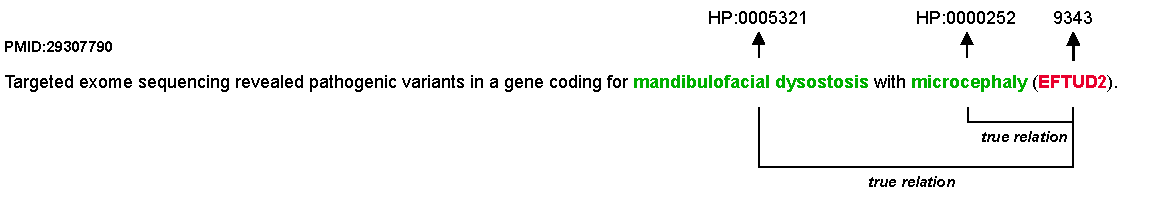
\includegraphics[width=\linewidth]{images/chapter_4/example_paper_knowledge_graph.pdf}}
\caption[Example of an Annotated Sentence]{An example of an annotated sentence retrieved from the PGR-crowd dataset from article PMID:29307790. The phenotype entities are linked to the HPO ontology (HP:0005321 and HP:0000252), and the gene entity is linked to the NCBI gene database (9343). We simplified the sentence to facilitate reading comprehension.}
\label{fig:example}
\end{figure*}

The first step towards biomedical RE based on recommendation was to adapt three publicly available RE datasets into the standardized recommender systems format of $<$user-item-rating$>$. We chose the PGR-crowd \citep{sousa2020hybrid} dataset that describes relations between human phenotypes and genes (Figure~\ref{fig:example}), the DDI Corpus \citep{herrero2013ddi}) that describes relations between drugs/chemicals, and the BC5CDR Corpus \citep{li2016biocreative}, that describes drugs/chemicals interactions with diseases, to demonstrate the range of our approach.

To make the adaption of biomedical RE datasets to the $<$user-item-rating$>$ recommendation format, we had first to decide which entities would be considered the users (\textit{user} entities) and the items (\textit{item} entities), for the datasets that had different type entities (PGR-crowd and BC5CDR dataset). Our choices for \textit{item} entities, described in detail in Section III under the A. Datasets sub-section, were to give priority to entities that were covered by ontological KGs (phenotypes in the PGR-crowd by the HPO) and to diversify the type of ontological KGs chosen (the DO for diseases in the BC5CDR Corpus). Therefore, as KGs, we used the ontologies HPO \citep{kohler2019expansion}, ChEBI \citep{hastings2012chebi}, and DO \citep{schriml2012disease}, linked to the \textit{item} entities when possible. 

Figure~\ref{fig:pipeline} illustrates an example of a relation recommendation where the user \textit{EFTUD2} is related to \textit{Microcephaly} and \textit{Mandibulofacial dysostosis} in our RE dataset of reference (Figure~\ref{fig:example}). Using the KG we can determine that one of the ancestor connections for \textit{Microcephaly} and \textit{Mandibulofacial dysostosis} is \textit{Abnormality of the skull}. By sharing an ancestor connection, these two items reinforce the connection between other descendants and the user \textit{EFTUD2}. Thus, we can recommend a relation between our user \textit{EFTUD2} and our item \textit{Cephalocele} (i.e., the green dashed line).

\begin{figure}[!h]
\centerline{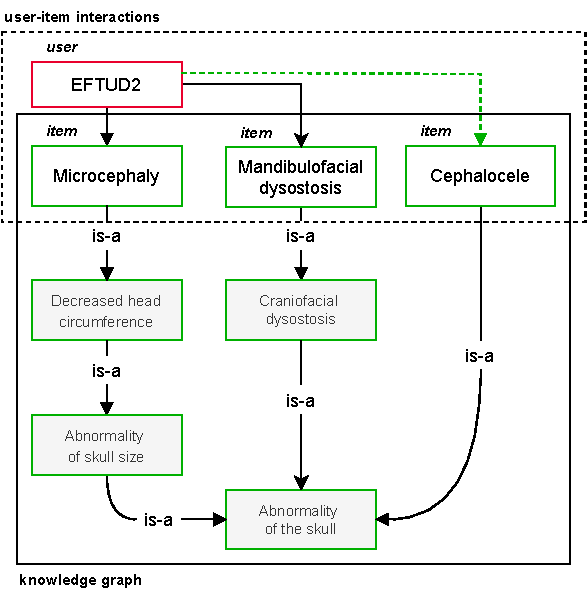
\includegraphics[width=0.6\textwidth]{images/chapter_4/paper_knowledge_graph.pdf}}
\caption[Example of a Relation Recommendation]{An example of a relation recommendation retrieved from the adapted PGR-crowd dataset \citep{sousa2020hybrid}. This example illustrates how a graph connection can contribute to a new relation recommendation.}
\label{fig:pipeline}
\end{figure}

In real-case scenarios, our approach would imply adapting existing and future RE biomedical datasets so that all entities are linked to a KG identifier, which by itself would enhance the applicability of such datasets. Moreover, linking identified entities to KGs is already a widely disseminated NLP task called Named-Entity Linking (NEL) or Concept/Entity Normalization, and most of the time, a natural precedent to RE \citep{huang2020biomedical}. As stated previously, a large volume of biomedical ontologies covers most types of studied entities. Therefore, the biggest hurdle would be to guarantee high KG coverage for the original datasets, while our adaptation of the datasets to a recommendation format is highly generalizable. For instance, given a biomedical sentence within a dataset, where the offsets of the entities of interest are identified and linked to KGs (Figure~\ref{fig:example}), the next step would be to give a rating to the possible relations considering the whole training dataset and identifying if there are other entities within the KG ancestry line that exhibit similar relations that can further support a true relation. Thus, we expect that the degree of coverage of each KG over each dataset dictates the effectiveness of the approach as well as other factors that we will discuss throughout this manuscript. 

After dataset re-formation, we adapted a state-of-the-art recommendation system to recommend relations between biomedical entities considering the specificities of the domain and evaluated the system's added value to a standard state-of-the-art deep learning biomedical RE system. 

In this paper, we present the results for relation recommendation on its own and then the added value of these recommendations to a deep learning biomedical RE system. Our results show that adding KG-based recommendations improves RE systems' ability to identify true relations in high KG coverage settings that baseline deep RE models could not extract from the text, indicating that the recommendation model adds value to the RE task. This work resulted in the following main contributions:

\begin{itemize}
    \item Pipeline for integrating a KG-based recommendation model in a biomedical RE system, including the adaptation of RE datasets for training. 
    \item Biomedical RE deep learning system with added knowledge in the form of KG-based recommendations (K-BiOnt).
\end{itemize}

The following section will present the related work for RE and recommender systems that specifically target the biomedical domain. We will then proceed to methodology, where we describe the dataset construction and the different training stages on their own and their joint evaluation. Next, we present results and discuss the effects of the KG-based recommendation on biomedical RE. Finally, we finish with the main conclusions and future work. 


\section{Related Work}

Biomedical RE is a task in NLP that usually follows Named-Entity Recognition (NER) and Named-Entity Linking (NEL) or Concept/Entity Normalization \citep{funk2014large}, the identification and mapping of entities in unstructured text, respectively \citep{sousa2021using}. This information extraction task mostly focuses on relations within the same sentence \citep{PMID:32032717}, with approaches that range from co-occurrence to a variety of Machine Learning methods. However, in recent years, deep learning approaches have become state-of-the-art for most domains achieving high levels of precision.
However, many biomedical relations are still hard to extract even when exploring the full documents \citep{verga-etal-2018-simultaneously}.
This can be explained by the complexity of the domain that requires extensive domain knowledge to be correctly perceived. 
One of those models, inspired by the BO-LSTM and BI-LSTM models \citep{lamurias2019bo,xu2018leveraging} is the BiOnt model \citep{sousa2020biont}. The BiOnt model uses deep learning methods along with domain-specific ontologies, achieving state-of-the-art results. Thus, it is a model that already explores external sources of knowledge to perform biomedical RE, even if with less KG depth than our proposal. Therefore, in this work, we propose a more in-depth use of KGs with recommendation approaches to detect missed true annotations by BiOnt, which we detail in the methodology section. We chose BiOnt over other biomedical or even non-biomedical \citep{devlin2019bert,gu2021domain} RE systems \citep{lee2020biobert} due to its use of similar external entity knowledge. If we can effectively improve the BiOnt model, it shows that their use of knowledge is not sufficient to fully grasp less frequent relations. Nevertheless, we also use the state-of-the-art BioBERT system \citep{lee2020biobert} on the same datasets to provide an extra comparison baseline. The BioBERT system is a BERT-based contextualized word representation model based on a masked language model and pre-trained using bidirectional transformers on large-scale biomedical corpora. 

Item recommendation initially focused on similarity-based methods that aimed at extracting features of users and items, computing their similarity, recommending similar users or items to a target user. Similarity-based methods using Neural Network (NN) models effectively extract latent features of users and items for recommendations \citep{10.1145/2959100.2959190,10.1145/3109859.3109872,huang2020efficient}. However, they deal with issues such as data sparsity \citep{guo2017resolving}, cold-start \citep{10.1145/3397271.3401426}, and lack of explainability \citep{10.1145/3397271.3401032} (i.e., an user understanding why an item is being recommended). Content-based methods introduce additional information, such as relational data \citep{10.1145/3309547} and knowledge graphs \citep{ai2018learning,10.1145/3308558.3313411}, and help relieve those issues. Therefore, recently, researchers have focused their attention on generating recommendations using knowledge graphs as additional information \citep{9216015,10.1145/3397271.3401428}, such as the TUP system created by \cite{10.1145/3308558.3313705}.

Current recommender systems that deal with biomedical data target different tasks, such as recommending ontologies to annotate biomedical text \citep{martinez2017ncbo}, model biological processes \citep{wang2020independent}, recommending drugs to target SARS-CoV-2 regarding the COVID-19 pandemic \citep{info:doi/10.2196/21169}, recommending entities of potential interest to specific researchers \citep{barros2019using}, or even recommending articles to expand existing biomedical datasets \citep{PATRA2020103399}. There is also a focus on recommending articles and venues to researchers to limit their search space \citep{PMID:30441232, info:doi/10.2196/12957}, for instance, by performing keyword-based recommendation \citep{yang2018keyword}. Further, there is a significant amount of work done on biomedical KG completion \citep{zhang2021drug,fei2020enriching,biswas2019relation}, including trying to depend less on domain-specific labelling and going through a minimum supervision route that can scale with the volume of literature available \citep{yuan2020constructing}. 


\section{Methodology}

To demonstrate the benefits of allying KG-based Recommendation to deep Biomedical RE, we used three publicly available datasets describing relations between different types of biomedical entities: the PGR-crowd \citep{sousa2020hybrid,sousa2019silver}, the DDI Corpus \citep{herrero2013ddi}, and the BC5CDR Corpus \citep{li2016biocreative}. The first step was to convert these RE datasets into a format compatible with KG-based Recommendation, which required several adjustments and rating assessments described in detail in the following section. Moreover, in this section, we will provide the training and evaluation details for each component system: deep biomedical RE and KG-based Recommendation on their own and as added features in a deep biomedical RE system plus recommendations. All baseline systems used or adapted throughout our work are openly available through their respective authors, including original configuration details.   

%here
\subsection{Datasets}

To take advantage of KG-based Recommendation into RE, we had to create standard $<$user-item-rating$>$ datasets using the PGR-crowd, DDI Corpus, and BC5CDR Corpus original RE datasets. These datasets describe relations between human phenotypes and genes, using NCBI gene database\footnote{\url{https://www.ncbi.nlm.nih.gov/gene}} and HPO identifiers (PGR-crowd), between drugs/chemicals, that can be linked to ChEBI ontology identifiers (DDI Corpus), and interactions between drugs/chemicals and diseases, that can be linked to the ChEBI and DO ontologies (BC5CDR Corpus). The PGR-crowd and DDI datasets are available in the same XML format, and the BC5CDR Corpus is available in a text format for standard RE applications. Table~\ref{tab:dl_statistics} presents the RE datasets' general statistics, including counts for the total number of entity annotations and the distribution of true and false relations. A relation is considered true if semantically there is an implication of an association between two entities considered in the same sentence, and false if there is no semantic relation or a semantic connection negates the relation between the entities. We did not consider the DDI Corpus relations' different label classifications for this work, only the binary classification of true/false. 

\begin{table}[h]
\centering
  \caption[Statistics of PGR-crowd, DDI Corpus, and BC5CDR Corpus Regarding Relation Extraction]{Statistics of PGR-crowd, DDI Corpus, and BC5CDR Corpus regarding Relation Extraction}
  \label{tab:dl_statistics}
  \begin{tabular}{lcccc}
    \hline
    \multirow{2}{*}{Dataset} & \multirow{2}{*}{Annotations} & \multicolumn{3}{c}{Relations} \\
    \cline{3-5}
    & & True & False & Total \\
    \hline
    PGR-crowd & 4150 & 5501 & 626 & 6127 \\
    DDI Corpus & 18491 & 5000 & 29449 & 34449 \\
    BC5CDR Corpus & 32527 & 1448 & 2294 & 3742 \\
    \hline
  \end{tabular}
\end{table}

Although the protocols were similar for the three datasets, we had to consider that in the PGR-crowd and BC5CDR datasets, each relation had two distinct entities (genes and human phenotypes, and drugs/chemicals and diseases, respectively). To cast our \textit{item} roles for the PGR dataset, we chose the phenotype entities since these were already mapped to an ontological knowledge graph (HPO). To diversify our approach, for the BC5CDR Corpus, we decided to map disease entities to the DO ontology as \textit{item} entities. While on the DDI Corpus dataset, we were dealing with relations between the same type of entities (i.e., drugs/chemicals) that could both be mapped to a knowledge graph (ChEBI). 

In the PGR-crowd dataset, we considered our \textit{users} as genes and our \textit{items} as human phenotypes. Each relation can appear more than once in a RE dataset since different sentences/articles can describe the same relation. We can have multiple instances of the same relation with the same or different labels. Therefore, we attributed $1$ to true relations and $-1$ to false relations and considered the rating the sum of all occurrences of the same relation within the training dataset. This process allowed us to have only one occurrence of each relation as expected in recommender systems type datasets, where the user only rates an item once. Figure~\ref{fig:datasets} further elucidates the process by direct comparison with an example of the MovieLens-1m dataset \citep{10.1145/2827872}. We followed the same procedure for the BC5CDR Corpus, where we considered our \textit{users} drugs/chemicals and our \textit{items} diseases.

\begin{figure}[!h]
\centerline{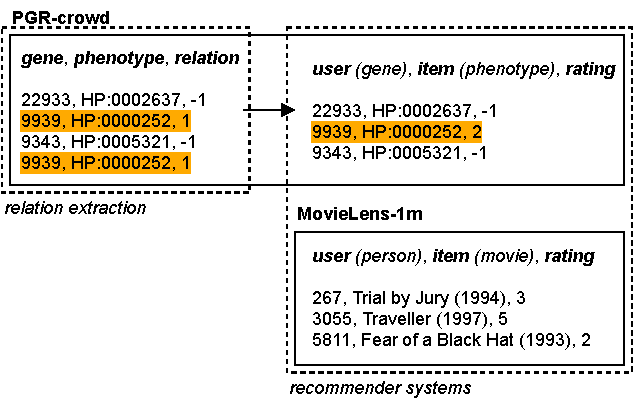
\includegraphics[width=0.6\textwidth]{images/chapter_4/datasets.pdf}}
\caption[Conversion from a Relation Extraction Type Dataset to a Recommender System Type Dataset]{The conversion from a relation extraction type dataset to a recommender system type dataset (PGR-crowd), including the comparison with examples from the MovieLens-1m dataset \citep{10.1145/2827872}.}
\label{fig:datasets}
\end{figure}

The DDI Corpus was not as straightforward to assign \textit{user} and \textit{item} roles to the drug/chemical entities. As each relation has two entities of the same type, we had to verify the symmetry between relations (e.g., is entity one an effect of entity two and vice-versa, or is it just a one-sided relationship?). For this, we considered the classification done by the creators of the DDI Corpus dataset, where each true relation could be of type \textit{effect} (asymmetric), \textit{mechanism} (asymmetric), \textit{advice} (symmetric), or \textit{int} (symmetric).  While the other types are intuitive, the \textit{int} type refers to the default positive interaction for which there is no additional information. So, we disregarded the entities' order for false and symmetric relations and maintained the order assigned for true asymmetric relations when adapting the RE dataset for recommendation. The process of calculating the ratings was identical to the previously described for the PGR-crowd and BC5CDR datasets. 

For model training, we converted all entities to an internal identifier. Also, the existing ratings were treated as positive interactions, while negative interactions were generated randomly by corrupting items following other models that target implicit feedback \citep{Wang_Wang_Xu_He_Cao_Chua_2019}. In the work done by \cite{10.1145/3308558.3313705}, the negative sampling was done by corrupting items that were less commonly used by users, which could not be applied to datasets with low average ratings. 

While previous works \citep{10.1145/2899005,bhargava2019collaborative} mapped publicly available datasets such as MovieLens-1m \citep{10.1145/2827872} and DBbook2014\footnote{\url{http://2014.eswc-conferences.org/important-dates/call-RecSys.html}} to DBPedia \citep{lehmann2015dbpedia} entities, whenever a mapping was available, we mapped our datasets to three publicly available biomedical ontologies (HPO for PGR-crowd, ChEBI for DDI Corpus, and DO for BC5CDR Corpus). For the PGR-crowd dataset, since the preexisting entity identifiers already linked to HPO, our coverage was 100\%. However, for the other two datasets (BC5CDR and DDI), the coverage was 26.0\% and 47.8\%, respectively, which is expected since the creators did not rely on the DO or ChEBI ontology to identify the original entities. The mapping was done automatically by exact matching, allowing for a Levenshtein distance of 1. Thus, particularly in the DDI and BC5CDR Corpora, we did not match possible synonym entities. Doing a more detailed mapping would require either the usage of external normalization tools \citep{funk2014large} or domain expertise to review all entities, which would be time and cost-intensive. However, we recognize the limitation in our entity normalization stage that could be improved in future work. In contrast with previous work \citep{10.1145/3308558.3313705}, we did not preprocess the datasets to filter low-frequency users and items or performed editing on the type of entities or relations in triples due to our universe being considerably smaller and the reassurance of using domain-specific ontologies instead of the generic domain of DBPedia. 

Table~\ref{tab:rs_statistics} describes the statistics for the three datasets (PGR-crowd, DDI Corpus, and BC5CDR Corpus) regarding the KG-based recommendation format. The data sparsity issue is prevalent in all datasets due to the low number of average ratings.

\begin{table}[h]
\centering
  \caption[Statistics of PGR-crowd, DDI Corpus, and BC5CDR Corpus Regarding Knowledge Graph-based Recommendation]{Statistics of PGR-crowd, DDI Corpus, and BC5CDR Corpus regarding Knowledge Graph-based Recommendation}
  \begin{tabular}{llccc}
    \hline
    && PGR-crowd & DDI Corpus & BC5CDR Corpus\\
    \hline
    \multirow{5}{*}{User-Item Interactions} & Users & 2176 & 2538 & 593 \\
    & Items & 409 & 2563 & 599 \\
    & Ratings & 4308 & 25973 & 2080 \\
    & Average Ratings & 2 & 10 & 4 \\
    & Sparsity & 99.5\% & 99.6\% & 99.4\% \\
    \hline
    \multirow{2}{*}{Knowledge Graph} & Entity & 15671 & 497046 & 13355 \\
    & Relation & 1 & 1 & 1 \\
    \hline
    \multirow{2}{*}{Multi-Tasks} & Item-Entity Alignments & 409 & 1225 & 156\\
    & Coverage & 100\% & 47.8\% & 26.0\%\\
    \hline
  \end{tabular}
  \label{tab:rs_statistics}
\end{table}

\subsection{Training}

The deep biomedical RE system BiOnt \citep{sousa2020biont} worked as our baseline since it achieved state-of-the-art performance in the datasets used in this work and also uses knowledge graphs as added information layers. We designed experiments regarding relation recommendation, following the work of \cite{10.1145/3308558.3313705}, and the incorporation of those recommendations into BiOnt (K-BiOnt). These systems were chosen due to their state-of-the-art results but also their availability and in-depth documentation. For all our experiments, we divided the datasets into a 6:1:3 ratio corresponding to the training set, the validation set, and the test set, respectively. We used the original datasets as provided for the Deep Learning component, making the appropriate parsing for the system specifications. While for the Recommendation component, we used the re-formatted datasets, as described in the previous sub-section. 


\subsubsection{Baseline Deep Learning Model}

The BiOnt model uses ontologies as external sources of knowledge to add information layers to a baseline deep learning model, following the work of \cite{lamurias2019bo}. An ontology is a formal definition of concepts related to a specific subject. It can be represented by a tuple $<C, R>$, where $C$ represents the set of concepts in an ontology and $R$ is the set of relations between the same ontology concepts. Similar to our dataset construction, the type of ontology relations considered by \cite{sousa2020biont} is subsumption relations, \textit{is-a} due to its transitive aspect. For instance, with $(c_1, c_2) \in R$, and $(c_2, c_3) \in R$, the authors assume that $(c_1, c_3)$ is a valid relation within the ontology. The ancestors of each concept $c$ are given by:

\begin{equation}
Anc(c) = a : (c, a) \in T
\label{equation:ancestors}
\end{equation}

where $T$ is the transitive closure of $R$. The authors define the common ancestors between the concepts $c_1$ and $c_2$ as:

\begin{equation}
CommRA(c_1, c_2) = Anc(c_1) \cap Anc(c_2)
\label{equation:commonancestors}
\end{equation}

A relation between different ontology concepts can be represented by $(x_1, y_1)$, where $x_1 \in X$ and $X$ represents the set of concepts in the first ontology and $y_1 \in Y$ and $Y$ represents the set of concepts in the second ontology. For instance, with $(x_2, y_2) \in RA$, where $RA$ is the set of relations between ancestors, and $(x_2\,\textit{is-a}\,x_1)$, and $(y_2\,\textit{is-a}\,y_1)$, their model assumes that $(x_1, y_1)$ is a valid relation. The concatenation of the relations between the ancestors of concepts $x_2$ and $y_2$ is defined using:

\begin{equation}
ConcRA(x_2, y_2) = Anc(x_2) \Join Anc(y_2)
\label{equation:cancestors}
\end{equation}

Since the common ancestors' channel could only be used for relations between the same type of biomedical entities (i.e., DDI Corpus), we only use the concatenation of ancestors channel for the relations between different biomedical entities (i.e., PGR-crowd). 

Each ontology concept corresponds to a one-hot vector $v_c$, a vector of zeros, except for the position corresponding to the concepts' ID. An embedding matrix $M \in \mathbb{R}^{D \times C}$ transforms these sparse vectors into dense vectors, where $D$ is the dimensionality of the embedding layer and $C$ is the number of concepts of the ontologies. Then, the output of the embedding layer is given by:

\begin{equation}
f(c) = M \cdot v_c
\label{equation:ontologyembedding}
\end{equation}

Next, the ontology embedding layer, with a dimensionality of 50 (as suggested by \cite{lamurias2019bo}), initializes its values randomly to be later tuned through back-propagation. Then, the vectors' sequence representing the relations between the ancestors of the terms is fed into a Long short-term memory (LSTM) layer, ordered from the more general concepts to the terms themselves. Finally, the system uses a max pool layer fed into a dense layer through a sigmoid activation function, and a softmax layer outputs the probability for each class.

The model was trained using a stochastic gradient descent optimization algorithm where weights were updated using the back-propagation of error algorithm. At each iteration, the model with a given set of weights creates predictions and computes the error for those predictions. The optimization algorithm seeks to alter the weights to reduce that error in the next evaluation. The relevant hyperparameters of this model tuned for our experiments were mini-batch gradient descent optimization algorithm (RMSprop), learning rate (0.0001), loss function (categorical cross-entropy), and dropout rate (0.500) for every layer except the penultimate and output layers.

We used the three standard evaluation metrics for RE models:
\textit{Precision}: Expresses how often the results are correct;
\textit{Recall}: It is the number of correct results identified;
\textit{F1 score}: Expresses overall performance by the harmonic mean of precision and recall.


\subsubsection{Item Recommendation} 

The TUP model created by \cite{10.1145/3308558.3313705} takes a list of user-item pairs $\mathcal{Y} = {(u, i)}$ as input, and outputs a relevance score $g(u, i; p)$, indicating the likelihood that $u$ likes $i$, given the preference $p \in \mathcal{P}$. In this work, instead of the terminology being \textit{the likelihood that $u$ likes $i$} is the likelihood that $u$ as a biomedical entity is related to $i$ as another biomedical entity. 
For each user-item pair, the TUP model induces a preference. The authors designed two strategies for preference induction: a hard approach that selects one out of the $P$ preferences and a soft way that combines all preferences with attentions. The soft strategy yielded a better performance for both authors' datasets. Therefore, we opted for this strategy to create our models. The preferences constitute the motives for each an \textit{user} entity may be connected to an \textit{item} entity. For traditional recommendation set-ups, these usually lack depth in explainability. To avoid that, in this work, we provided them explicit semantics by aligning them with the KG relations, capturing the intuition that the types of item attributes play a crucial role in user assignment. Considering that an entity might be related to another entity according to various factors, which can not be restricted by a firm boundary, instead of selecting the most prominent preference, the soft strategy combines multiple preferences via an attention mechanism:

\begin{equation}
p = \sum_{p' \in \mathcal{P}} \alpha_{p'} p'
\label{equation:soft}
\end{equation}

where $\alpha_{p'}$ is the attention weight of preference $p'$, and defined as proportional to the similarity score:

\begin{equation}
\alpha_{p'} \propto \phi(u, o, p')
\label{equation:similarity}
\end{equation}

To deal with the issue where one entity (i.e., \textit{user}) might be associated with multiple entities (i.e., \textit{items}), and also, several entities (i.e., \textit{users}) may be associated with a single entity (i.e., \textit{item}) (1-to-N and N-to-1 issues), the authors introduce preference hyperplanes assigning each preference with two vectors (inspired by TransH \citep{10.5555/2893873.2894046}): $w_p$ for the projection to a hyperplane, $p$ for the translation between users and items. The authors define the hyperplane-based translation function as follows:

\begin{gather}
g(u, i; p) = \| u^{\perp} + p - i^{\perp} \| \\
u^{\perp} = u - w_p^T u w_p, \quad
i^{\perp} = i - w_p^T i w_p   
\label{equation:hyperplane}
\end{gather}
 
where $u^{\perp}$ and $i^{\perp}$ are projected vectors of the user and the item and are obtained through the induced preference $p$. $w_p$ is the projection vector that is obtained along with the induction process of preferences $p$ through attentive addition of all projection vectors based on the induced attention weights in the soft strategy:

\begin{equation}
w_p = \sum_{p' \in \mathcal{P}} \alpha_{p'} p' w_{p'}
\label{equation:wp}
\end{equation}

Then, the authors encourage the translation distances of the interacted items to be smaller than random ones for each user through the  Bayesian Personalized Ranking (BPR) Loss function:

\begin{equation}
\mathcal{L}_p = \sum_{(u, i) \in \mathcal{Y}} \sum_{(u, i') \in \mathcal{Y}'} - \log \sigma [g(u, i'; p') - g(u, i; p)]
\label{equation:ir}
\end{equation}

where $\mathcal{Y}'$ contains negative interactions by randomly corrupting an interacted item to a non-interacted one for each user. 

The relevant hyperparameters for TUP tuned for our experiments were learning rate (0.005), $L_2$ coefficient ($10^{-5}$), optimization method (Adagrad), batch size (512), embedding size (64), and the number of preferences (1). The number of preferences corresponds to the number of different relations within the KGs attributed to each dataset (Table~\ref{tab:rs_statistics}). Since this model is inspired by the TransH model described previously, some functionalities could not be explored due to the lack of relation diversity. 

The TUP model uses as evaluation metrics the following:

\begin{itemize}
    \item \textit{Precision@10}: The fraction of the of \textit{item} entities recommended that are relevant for establishing relations with our \textit{user} entities, within the top 10 recommendations. The final precision corresponds to the mean of all \textit{user} entities. 
    \item \textit{Recall@10}: The proportion of \textit{item} entities relevant to the \textit{user} entities that have been successfully recommended within the top 10 recommendations. The final recall corresponds to the mean of all \textit{user} entities. 
    \item \textit{F1 score@10}: The harmonic mean of precision at rank 10 and recall at rank 10. 
    \item \textit{Hit ratio@10}: It is 1 if the gold \textit{item} entities are recommended within the top 10 \textit{item} entities, otherwise it is 0. The final hit ratio score corresponds to the mean of all \textit{user} entities.  
    \item \textit{nDCG@10}: The Normalized Discounted Cumulative Gain (nDCG) is a standard measure of ranking quality that considers the graded relevance among positive and negative \textit{item} entities within the top 10 of the ranked list. 
\end{itemize}

\subsubsection{K-BiOnt}

The general approach pipeline that joins BiOnt to a TUP adaptation for RE is presented in Figure~\ref{fig:full_pipeline}.

\begin{figure*}[!h]
\centerline{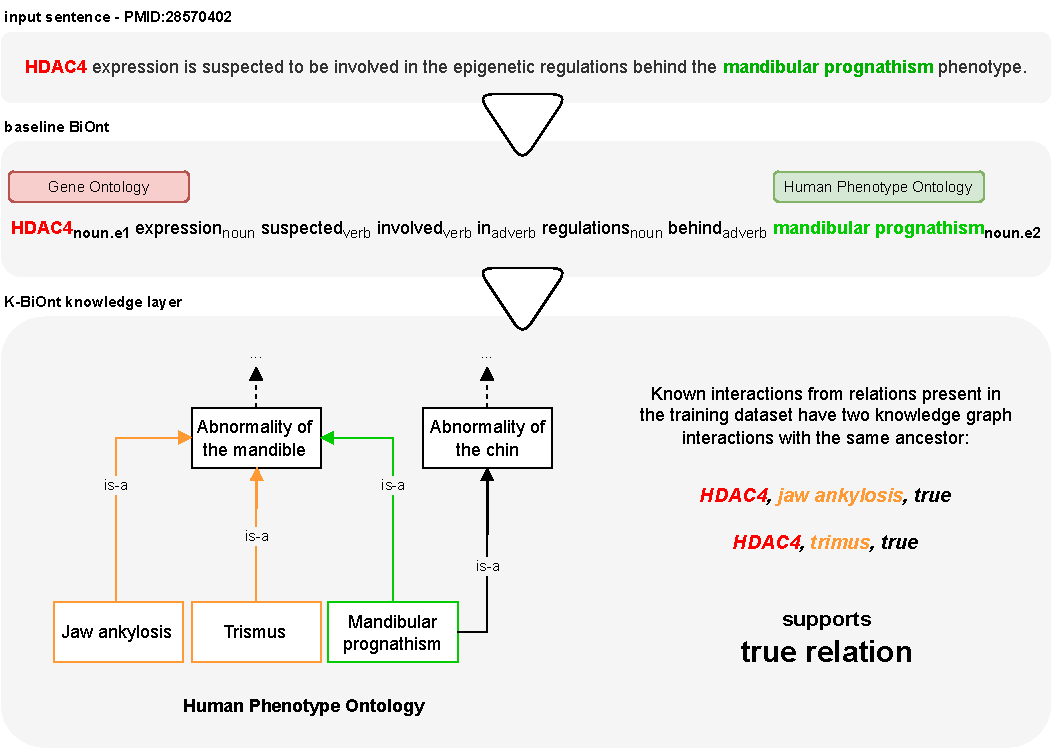
\includegraphics[width=\linewidth]{images/chapter_4/pipeline.pdf}}
\caption[General K-BiOnt Approach Pipeline]{General approach pipeline regarding the joint approaches BiOnt and the knowledge layer based on recommendation. We simplified the input sentence to facilitate reading comprehension (PMID:28570402).}
\label{fig:full_pipeline}
\end{figure*}

First, we proceed with the standard training process of the BiOnt model, which can be divided into three main stages after sentence tokenization: WordNet classes \citep{ciaramita2006broad}, word embeddings, and ontology embeddings. The ontology embedding stage represents the relations between the ancestors for each ontology concept corresponding to an entity. For instance, for the PGR-crowd dataset, the system links the entities to the HPO and GO biomedical ontologies, the DDI Corpus to the ChEBI ontology, and the BC5CDR Corpus to the ChEBI and DO ontologies with different coverage degrees, as discussed previously. The system uses a max pool layer fed into a dense layer through a sigmoid activation function, and a softmax layer outputs the probability for each class. The BiOnt model adds external entity knowledge through two channels of common ancestry and concatenation of ancestors. These knowledge channels aim to answer the questions: i) Do the entities in question share ancestors? (only applicable to relations between the same type of entities); and ii) Do the entities in question have ancestors that have established relations? The BiOnt model uses the answer to these two questions to support or discard a relation. However, our K-BiOnt knowledge layer goes deeper into the inferences that can support or discard a relation by answering: Do we have entities outside of the ones considered in the relation that we know that establish relations with one of the entities' ancestors? If yes, how many? In what capacity (true/negative)? And to what degree (e.g., 2, 3, or -5)? 


Thus, going back to the example in Figure~\ref{fig:full_pipeline}, our goal is to support or discard a relation between a gene \textit{HDAC4} and a human phenotype, \textit{Mandibular prognathism}. Yet, since their ancestors do not have known relations (excluding the BiOnt concatenation of ancestors' channel) and the entities are from different types (excluding the usage of the common ancestors' channel), the BiOnt knowledge layer does not provide information to support or discard this relation. However, since we know from the training set that the gene, \textit{HDAC4}, shares a true relation with both the \textit{Jaw ankylosis} and the \textit{Trimus} phenotype, and both of these entities have the same ancestor as the \textit{Mandibular prognathism} phenotype, we can support a true relation between \textit{HDAC4} and \textit{Mandibular prognathism}. Our knowledge layer considers translational relationships between \textit{users} and \textit{items}. This, in our example, means that for each human phenotype (\textit{item}) related to a gene (\textit{user}), we consider the whole subsequent ancestry of the phenotype until root to provide information on our gene.  


\subsection{Joint Evaluation}

To evaluate our approach, we created a confusion matrix table to compare the BiOnt model's output and the adjusted TUP model results against our gold standard test sets. This table served as a way for us to detect the main contributions of adding KG-based recommendation to a deep RE model (K-BiOnt) to all datasets.

One caveat is that an extracted relation between two entities is specific to the text where they are mentioned; however, in KG-based recommendation, the relation tag is specific to the entities it refers to. To overcome this issue, we primarily considered the label generated through the application of the baseline system to the normal text-bound RE dataset. We only changed the output if the modules (Deep Learning and Recommendation) disagreed with the label. Upon disagreement, we only altered the label if the Recommendation module assigned true and the baseline system false. Thus, only considering the Recommendation module input to capture an undetected connection.   
Table~\ref{tab:cross_validation} presents an example of a confusion matrix table for five distinct scenarios using relations from the PGR-crowd dataset. All true relations captured by KG-based recommendation were attributed with the final judgment of true independently of the Top@N. We only considered false relations in the final judgment if all model components agreed on the label false. Therefore, the BiOnt module component was preferred for the attributed label since it is based on the linguistic context of the relationship. The Recommendation module, based exclusively on knowledge regarding the target entities, was only considered for potential true labels that we hypothesize could not be retrieved solely on the linguistic context or were less frequent in the training data. 

\begin{table}[h]
\centering
  \caption[Confusion Matrix Example for Different K-BiOnt Scenarios]{An example of a confusion matrix table for five distinct scenarios using relations from the PGR-crowd dataset. FJ stands for Final Judgement and GS for Gold Standard}
  \begin{tabular}{lcccccc}
    \hline
    Relation (user-item) & BiOnt & Top@3 & Top@5 & Top@10 & FJ & GS\\
    \hline
    WNT7B-cancer & True & True & True & True & True & True \\
    \hline
    Adcy1-seizures & False & False & False & True & True & True \\
    \hline
    TRAPPC2-developmental delay & True & False & False & False & True & True \\
    \hline
    \rowcolor[gray]{0.9}
    IARS2-neuropathy & False & False & False & False & False & True \\
    \hline
    \rowcolor[gray]{0.9}
    SLC12A6-autosomal recessive & False & True & True & True & True & False \\
    \hline
  \end{tabular}
    \label{tab:cross_validation}
\end{table}

\section{Results and Discussion}

This section presents our assessment of the benefits of using KG-based recommendation as an added resource for RE systems in the biomedical domain. As a baseline, we compared the results of the baselines deep learning models BiOnt \citep{sousa2020biont} and BioBERT \citep{lee2020biobert} for RE with the adjusted TUP model \citep{10.1145/3308558.3313705} for item recommendation and the integration of BiOnt with TUP (K-BiOnt).


\subsection{Deep Learning Model}

Table~\ref{tab:biont_results} presents the results for the application of our three datasets to the deep learning models BiOnt and BioBERT. 

For BiOnt, the results were slightly different from the performances reported on the original work for the DDI Corpus \citep{herrero2013ddi}, but almost identical for the PGR-crowd dataset \citep{sousa2020hybrid}. We can justify the DDI Corpus performance differences ($\approx$ 4\% in F1) with our use of the updated ChEBI version that has fewer alignments with the entities in the original dataset. The PGR-crowd has a significant imbalance of true/false relations, with the majority of relations being true and the DDI and BC5CDR Corpora share the same imbalance but in favour of the false relations (Table~\ref{tab:dl_statistics}), which can affect the performance of these datasets differently, despite the BiOnt model ability to assign class weights.

As for the BioBERT system's PGR-crowd dataset and the BC5CDR Corpus results were very similar to the BiOnt's model performance. However, given the class imbalances of all three datasets, it should be possible to alter class weights. Still, BioBERT's loss function does not allow this flexibility, possibly undermining their results. The BioBERT system significantly outperformed the BiOnt model for the DDI Corpus, despite the class imbalances. 

\begin{table}[h]
\centering
  \caption[Results for Relation Extraction using BiOnt and BioBERT Systems]{Overall results regarding the BiOnt and BioBERT systems. P stands for Precision, and R for Recall}
  \label{tab:biont_results}
  \begin{tabular}{llccc}
    \hline
    Dataset & System & P (\%) & R (\%) & F1 (\%) \\
    \hline
    \multirow{2}{*}{PGR-crowd} & BioBERT & 80.04 & 99.22 & 88.60 \\
    & BiOnt & 81.30 & 97.55 & 88.69  \\
    \hline
    \multirow{2}{*}{DDI Corpus} & BioBERT & 86.61 & 87.23 & 86.92 \\
    & BiOnt & 61.85 & 73.24 & 67.06 \\
    \hline
    \multirow{2}{*}{BC5CDR Corpus} & BioBERT & 59.78 & 72.67 & 65.60 \\
    & BiOnt & 63.96 & 71.73 & 67.62 \\
    \hline
  \end{tabular}
\end{table}


\subsection{Knowledge Graph-based Recommendation}

Table~\ref{tab:ir_results} presents the results for the adapted TUP model using the soft item recommendation strategy mentioned in Section 3.2.3. TUP authors \citep{10.1145/3308558.3313705} state that the peak performance for their model is when the average number of ratings for users ranges from 100 to 200. This range is far from our average number of ratings for both datasets (2 for PGR-crowd, 10 for DDI Corpus, and 4 for the BC5CDR Corpus). Thus, we believe that more training data allied with less sparsity would enhance our results further. Also, the higher overall results for the PGR-crowd demonstrate the importance of item-entity alignments since all items (i.e., human phenotypes) were linked to the HPO \citep{kohler2019expansion}. In contrast, on the DDI and BC5CDR Corpora, only 47.8\% and 26.0\% of the items could be linked to the ChEBI \citep{herrero2013ddi} and DO \citep{schriml2012disease} ontologies, respectively, leading to a drop in performance.  

\begin{table}[h]
\centering
  \caption[Results for Item Recommendation with TUP]{Overall results regarding the TUP model for Item Recommendation. P stands for Precision, and R for Recall}
  \label{tab:ir_results}
  \begin{tabular}{lccccc}
    \hline
    Dataset & P@10 (\%) & R@10 (\%) & F1@10 (\%) & Hit ratio@10 (\%) & nDCG@10 (\%) \\
    \hline
    PGR-crowd & 3.72 & 32.10 & 6.59 & 35.96 & 19.33 \\
    \hline
    DDI Corpus & 1.90 & 2.40 & 1.90 & 18.70 & 8.20 \\
    \hline
    BC5CDR Corpus & 0.53 & 2.24 & 0.79 & 5.28 & 2.37 \\
    \hline
  \end{tabular}
\end{table}


\subsection{Joint Evaluation}

Table~\ref{tab:final_results} presents the final results by adding the adjusted TUP model recommendation to the BiOnt model (K-BiOnt), considering  top@3, top@5, and top@10 recommendations. These results are a reflection of the results of the confusion matrix tables created as described in the example of Table~\ref{tab:cross_validation}.  

\begin{table}[h]
\centering
  \caption[K-BiOnt Final Results]{Final results by adding the adjusted TUP model recommendations to the BiOnt model (K-BiOnt), considering top@3, top@5, and top@10 recommendations. P stands for Precision, and R for Recall}
  \label{tab:final_results}
  \begin{tabular}{llccc}
    \hline
    Dataset & Configuration & P (\%) & R (\%) & F1 (\%) \\
    
    \hline
    \multirow{4}{*}{PGR-crowd} & BiOnt & \textbf{81.30} & 97.55 & 88.69 \\
    & + Top@3 & 81.23 & 97.90 & \textbf{88.79} \\
    & + Top@5 & 80.98 & \textbf{98.17} & 88.75 \\
    & + Top@10 & 80.98 & \textbf{98.17} & 88.75 \\
    
    \hline
    \multirow{4}{*}{DDI Corpus} & BiOnt & \textbf{61.85} & \textbf{73.24} & \textbf{67.06} \\
    & + Top@3 & 61.85 & 73.24 & 67.06 \\
    & + Top@5 & 61.85 & 73.24 & 67.06 \\
    & + Top@10 & 61.85 & 73.24 & 67.06 \\
    
    \hline
    \multirow{4}{*}{BC5CDR Corpus} & BiOnt & 63.96 & 71.73 & 67.62 \\
    & + Top@3 & 63.96 & 71.73 & 67.62  \\
    & + Top@5 & 64.15 & 72.34 & 68.00  \\
    & + Top@10 & \textbf{64.45} & \textbf{73.25} & \textbf{68.56} \\


    \hline
  \end{tabular}
\end{table}


For the PGR-crowd dataset, the average number of ratings per \textit{user} entity is 2. A false relation usually appears only once being rated with $-1$ and not a lower number, which is insufficient to indicate to the model that the \textit{user} entity is unrelated to an \textit{item} entity. An approach that we could study in the future is creating negative sampling using false relations, not the traditional random sampling for negative observations associated with implicit feedback. The added performance of TUP over the BiOnt model (K-BiOnt) holds for all Top@N. However, the number of false positive relations increases with the subsequent decrease in performance for Top@5 and Top@10. Although, after closer inspection to the added false positives, for the majority of them, the \textit{item} entity human phenotype is under the \textit{Mode of inheritance} category of HPO, not under \textit{Phenotypic abnormality}. This last branch is the most developed branch within the HPO and is of more interest to researchers. Likewise, the BC5CDR Corpus also increased performance compared to the BiOnt baseline for Top@5 and Top@10 despite the low TUP performance, which indicates potential for a more impactful approach following improvement in linking the entities to KG identifiers. 

For the DDI Corpus, the results are identical across all Top@N (the BioBERT baseline) since we could not capture a true positive through item recommendation within the first ten recommendations. 


\subsection{Ablation Study}

To study the impact of knowledge graph coverage, we chose the dataset with the lowest value in coverage (BC5CDR Corpus). We created the recommendation module only taking into account the 156 items linked to DO ontological concepts. Table~\ref{tab:final_results_ab} presents the results for this study. 

\begin{table}[h]
\centering
  \caption[Ablation Study Results Regarding the TUP model for Item Recommendation]{Ablation study results regarding the TUP model for Item Recommendation for the Full Dataset and the KG covered Subset of the BC5CDR Corpus. P stands for Precision and R for Recall}
  \label{tab:final_results_ab}
  \begin{tabular}{lccccc}
    \hline
    Dataset & P@10 (\%) & R@10 (\%) & F1@10 (\%) & Hit ratio@10 (\%) & nDCG@10 (\%) \\
    \hline
    Full BC5CDR & 0.53 & 2.24 & 0.79 & 5.28 & 2.37 \\
    \hline
    Subset BC5CDR & 0.79 & 4.87 & 1.32 & 7.92 & 5.62 \\
    \hline
  \end{tabular}
\end{table}

By Table~\ref{tab:final_results_ab}, we can verify that the presence of only ontological covered items, even if in a small number, is enough to impact the performance of item recommendation, almost doubling our previous results. Even if there was no significant impact on the K-Biont model due to the small number of items, we know that augmenting the covered items through a more robust concept normalization step can improve the K-BiOnt performance. 

\subsection{Impact on RE}

We decided to perform an error analysis on the performance of the PGR-crowd dataset, comparing the baselines BioBERT and BiOnt to our approach K-BiOnt to measure their actual impact on the RE task. We found that more true relations were identified by considering relations that the KG-based recommendation model recommended.  

In the PGR-crowd dataset, the \textit{item} entities (i.e., human phenotypes) are all linked to the HPO, with subsequent complete coverage of the KG entities over the \textit{item} entities. The full coverage translated to a higher contribution of the recommendation module to the RE task. Figure~\ref{fig:example_r} illustrates one of those true relations detected by the recommendation module and missed by the BiOnt model. Note that our models only added true relations recommended with the adjusted TUP at Top@3. All other experiments also recommended false positives, undermining the recommendation module benefits.

\begin{figure*}[!h]
\centerline{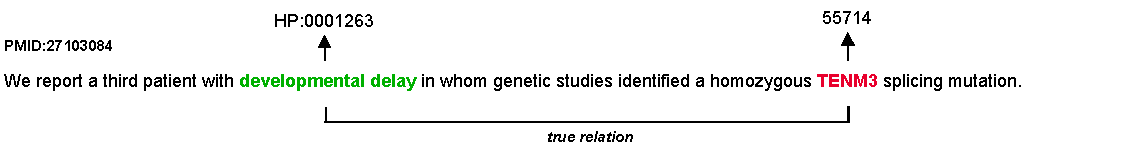
\includegraphics[width=\linewidth]{images/chapter_4/example.pdf}}
\caption[An Example of a True Relation Detected by the Recommendation Module]{An example of a true relation detected by the recommendation module from the PGR-crowd dataset from article PMID:27103084. The phenotype entity is linked to the HPO ontology (HP:0001263), and the gene entity is linked to the NCBI gene database (55714). We simplified the sentence to facilitate reading comprehension.}
\label{fig:example_r}
\end{figure*}

These results show the advantage of adding recommendations to RE, mainly to populate knowledge bases of gold standard relations, where the goal is not only to identify the relation that is explicitly mentioned in the text but to find every true relation that we can derive from it. The success of the recommendation module is explained by the exploration of KGs that allows the RE process to consider the connections between the associated KG.  

However, existing KGs are far from complete, limiting the knowledge we can transfer into RE systems. Considering this limitation, \cite{10.1145/3308558.3313705} aligned item recommendation (TUP) with KG completion (TransH). KG completion is a field in accelerated popularity given its relevance for question answering tasks \citep{10.1145/3132847.3132977,10.1145/3289600.3290956}, but also to search entities and their relations in text \citep{ji2020survey}. This field should be considered for future exploration of added knowledge to biomedical RE to further enhance the recommendation of less frequent relations.  


\section{Conclusion and Future Work}

This paper proposed a new recommendation-based complementary approach to deep learning biomedical RE that considers biomedical ontologies as additional sources of information. The KG-based recommendation pipeline presented in this work takes advantage of \textit{user} entity-\textit{item} entity interactions as well as knowledge graphs that can be linked to \textit{item} entities. In our case study, the biomedical KGs were HPO, ChEBI, and DO. We performed experiments using both item recommendation algorithm on its own and as an added module to a deep biomedical RE system. We present the benefits of using both methods simultaneously and the RE task's added value. Our results show that KG-based recommendations can be a valuable asset to biomedical RE by detecting previously undiscovered true relations between biomedical entities. However, the low coverage of the associated KGs damages performance.

Additionally, we produced three recommendation datasets in the format $<$user-item-rating$>$ for human phenotype and gene relations, drugs/chemicals interactions, and drugs/chemicals and diseases relations, attributing a rating for each user-item pair. We also presented a comprehensive pipeline for creating a biomedical RE system using KG-based recommendation (K-BiOnt). Ultimately, we demonstrated that adding recommendations can increase deep biomedical RE models' performance by considering external sources of knowledge when they have sufficient coverage of the domain.

Biomedical RE datasets usually do not describe more than one type of relation. However, upon the availability of a dataset describing more types of labelled relations, a multi-graph approach could be employed linking each \textit{item} entity to their respective ontological identifier. Even though we could argue that our representation of the ratings between user-item pairs is not representative of the real world, it is a cross-approach problem. Current deep learning approaches to biomedical RE also take labelled data to create models where the distribution is not a representation of real-world data and where a lot of less frequent associations are missed. 
In the future, the approach could be expanded by considering other types of relations between biomedical entities and by applying it to different types of baseline systems (i.e., BioBERT). Another angle to be explored could be adding more biomedical ontologies, including possible interconnections between multiple ontologies, that could expand our KGs even further by increasing the number of preferences. Also, upon availability within biomedical ontologies, another complementary route could be adding informative axioms such as \textit{disjointness} and studying the effect of ontological depth.